% ---------------------------- README -----------------------------------------
% This file holds section two of the body of the Machine Intelligence I script.
% -----------------------------------------------------------------------------

\newpage
\section{Learning Theory and Support Vector Machines}
\label{sec:learn-theory-supp}
\setcounter{equation}{0}

Statistical learning theory (SLT) provides a general mathematical
framework to describe and analyze learning problems. It allows to
identify conditions under which inductive learning is possible. It
provides bounds quantifying data requirements and limits to the
performance of a learning algorithm. Support Vector Machines (see
ch. \ref{sec:SVM}) have been developed in the framework of SLT and
represent a powerful learning algorithm based on the principle of
\underline{S}tructural \underline{R}isk \underline{M}inimization
(SRM).

% -----------------------------------------------------------------------------
\subsection{Elements of Statistical Learning Theory}

% -----------------------------------------------------------------------------
\subsubsection{Formulation of the Problem}
Learning can be understood as model selection with the goal of finding
a model of optimal (generalization) performance.\slideref{learning\\ as\\ model selection} The previous chapter described
inductive learning via \emph{empirical risk minimization} (ERM, see
\ref{sec:perf-meas-model}) -- SLT discusses when the ERM principle can
be expected to work. 

\begin{equation} \tag{generalization error}
	E_{[\vec{w}]}^G = \int d \vec{x} d y_T P_{(y_T, \vec{x})}
		e_{(y_T, \vec{x};\vec{w})} \eqexcl \min
\end{equation}
\[ \begin{array}{cl}
	\text{generalization error (mathematical expectation)} \\ \\
	\Downarrow \text{ \textbf{ERM} } \Downarrow 
		& \leftarrow \text{ When does this work?} \\\\
	\text{training error (empirical average)}
\end{array} \]
\begin{equation} \tag{training error}
	E_{[\vec{w}]}^T = \frac{1}{p} \sum_{\alpha = 1}^p 
		e_{(y_T^{(\alpha)}, \vec{x}^{(\alpha)}; \vec{w})} \eqexcl \min
\end{equation}
\paragraph{Change in Nomenclature}\mbox{} \\
\indent {\it (to be consistent with \cite{Vapnik1998})}
\[ \begin{array}{lll}
	E_{[\vec{w}]}^G 
		& \rightarrow R_{[\vec{w}]}
		& \text{(risk)} \\\\
	E_{[\vec{w}]}^T 
		& \rightarrow R_{\emp [\vec{w}]}
		& \text{(empirical risk)} \\\\
	e_{(y_T, \vec{x}; \vec{w})}
		& \rightarrow \underbrace{ Q_{[\vec{z}; \vec{w}]} }_{
				\text{data point; model}}
		& \text{(individual cost)}
\end{array} \]

\paragraph{The learning problem} 
\begin{itemize}
\item $p$ observations $\vec{z}^{(\alpha)}, \alpha = 1, \ldots, p$ drawn iid from  unknown distribution
\item \emph{stationarity:} training and test distributions are identical
\end{itemize}

\begin{figure}[h]
  \centering
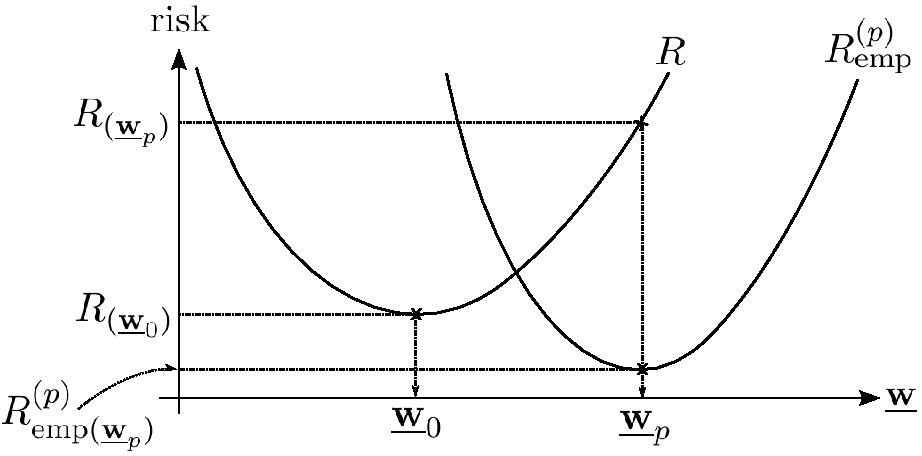
\includegraphics[height=6cm]{section2_fig1} 
  \caption{the learning problem}
\end{figure}



\paragraph{When does inductive learning through empirical risk minimization work?} \mbox{}
\\\\
\textbf{Goal:} Find conditions for which:
\begin{equation}
	\lim_{p \rightarrow \infty} P \Big\{ \big| R_{(\vec{w}_p)}
		- R_{(\vec{w}_0)} \big| \geq \eta \Big\} = 0 
		\text{ for all } \eta > 0
\end{equation}
\textbf{Requirement:} The ERM procedure should converge to the optimal predictor in the limit of infinite number of observations. 

\paragraph{How strongly does $R_{(\vec{w}_p)}$ differ from $R_{(\vec{w}_O)}$ for a finite sample?} \mbox{}
\\
For a given confidence $\epsilon$, find $\eta$ such that
\begin{equation}
	P \Big\{ \big| R_{(\vec{w}_0)} - R_{(\vec{w}_p)} \big| \geq \eta \Big\}
		< \epsilon
\end{equation}

% -----------------------------------------------------------------------------

\subsubsection{The Key Theorem of Learning Theory}
\[ \begin{array}{ll}
	\Lambda = \{ \vec{w} \}: & \text{set of all predictors} \\
	\Lambda_{(c)} \subset \Lambda: & \text{set of all ''bad'' predictors}
\end{array} \]
\begin{figure}[h]
  \centering
  \begin{tabular}[h]{c c}
	\includegraphics[height=4.5cm]{section2_fig2}  
& \raisebox{15mm}{$\times\times\times: \Lambda_{(c)} = \big\{ \vec{w}: R_{(\vec{w})} \geq c \big\}$} 
  \end{tabular}
  \caption{key theorem}
\end{figure}




Definition of \emph{strict consistency}:
\begin{equation}
	\lim_{p \rightarrow \infty} P \bigg\{ \Big| 
		\inf_{\vec{w} \in \Lambda_{(c)}} R_{\emp (\vec{w})}^{(p)}
		- \inf_{\vec{w} \in \Lambda_{(c)}} R_{(\vec{w})}
		\Big| \geq \eta \bigg\} = 0
\end{equation}
\[ \begin{array}{lcl}
	\text{strict consistency}
	& \substack{ \rightarrow \\ \nleftarrow}
	& \substack{ \text{inductive learning via ERM} \\
			\text{(eq. (2.1))} }
\end{array} \]
{\it proof: supplementary material}

\paragraph{Key theorem}\mbox{}
\\
Let $a \leq R_{(\vec{w})} \leq A$ for all $\vec{w} \in \Lambda$ and $P_{(\vec{z})} \in \Pi$, then:
\begin{equation}
	\begin{array}{c}
	\text{The ERM procedure is strictly consistent for } \Lambda 
		\text{ and } \Pi \\
	\Updownarrow \\
	\lim\limits_{p \rightarrow \infty} P \bigg\{ 
		\sup\limits_{\vec{w} \in \Lambda}
		\Big( R_{(\vec{w})} - R_{\emp (\vec{w})}^{(p)} \Big)
		> \eta \bigg\} = 0 \text{ for all } P_{(\vec{z})} \in \Pi
	\end{array}
\end{equation}
{\it proof: supplementary material}
\\\\
Learning by induction through ERM is linked to the uniform (one-sided) convergence of the empirical averages $R_{\emp (\vec{w})}^{(p)}$ to their mathematical expectations $R_{(\vec{w})}$.

\paragraph{Law of large numbers}\mbox{}
\\
{\it ''The sequence of means converges to the expectation of a random variable (if it exists) as the number $p$ of samples increases.''} 
\begin{itemize}
	\itR can only be applied if set of predictors has a finite number of 
		elements (use Hoeffding's inequality for bound on 	
		deviations)
	\itR extension to infinite sets (e.g. MLPs) necessary
	\itR characterization of sets of predictors by ''capacity measures'' 
		(since number of models is infinite)
\end{itemize}

\paragraph{Why does this matter?} The key theorem of SLT provides the
conditions under which one can expect to learn from examples. It gives
bounds telling how good we can expect our predictions to be. 
% -----------------------------------------------------------------------------

\subsubsection{An important example: Linear classifiers}
\textcite{Cover1965} computes bounds on the pattern-separating
capacity of hyperplanes and nonlinear decision surfaces. It
demonstrates that the probability of ambiguous generalization is large
unless the number of
training patterns exceeds the capacity of the classifier.\\\\
$\Rightarrow$ link between the capacity of a classifier (linear
classifier) and its generalisation performance (probability of
ambiguous generalization).  A related calculation of the capacity
of linear connectionist neurons can be found in \parencite[ch.~40.3]{MacKay2003}. 
\\\\
\emph{Set of classifiers:} binary connectionist neurons with 
$y = \sign (\vec{w}^T \vec{x})$
\begin{figure}[h]
  \centering
 \includegraphics[height=3cm]{section2_fig3}  
  \caption{binary connectionist neuron}
\end{figure}


Classification boundary: $\vec{w}^T \vec{x} = 0 \leadsto$ hyperplane
\begin{figure}[h]
  \centering
  \begin{tabular}[h]{c c c}
	\raisebox{-2.5cm}{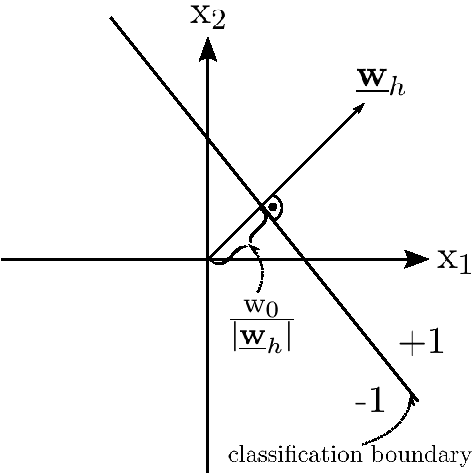
\includegraphics[height=6cm]{section2_fig4}}
	& \rule{5mm}{0pt}&$\vec{w} = \left(
          \begin{array}{c}
          \mathrm{w}_0 \\ \vec{w}_h
          \end{array}
          \right)
$
  \end{tabular}
  \caption{classification boundary induced by weight vector $\vec{w}_h$}
\end{figure}



\paragraph{Linear separability}
\[ \left. \begin{array}{l}
	\leadsto \text{classes do not overlap} \\
	\leadsto \text{classes can be separated by a hyperplane}
\end{array} \right \} \substack{ \text{all data points can be correctly} \\
				\text{classified by at least one classifier} \\
				\text{from the set} } \]

\paragraph{Statistics of linear separability} \mbox{}\\
\emph{Data:} observations $\vec{x}^{(\alpha)} \in \mathbb{R}^N, \alpha = 1, \ldots, p$, in general location\\
$\rightarrow$ (each subset of $N$ points should be linearly independent)
\begin{figure}[h]
  \centering
  \[ \begin{array}{lcl}
	\includegraphics[height=3.5cm]{section2_fig5}
	& \includegraphics[height=3.5cm]{section2_fig6}
	& 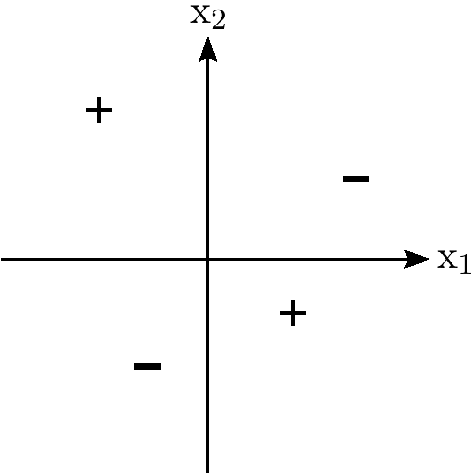
\includegraphics[height=3.5cm]{section2_fig7} \\
	\substack{ \text{four points in} \\ \text{general location} }
	& \substack{ \text{linearly separable assignment of} \\
			\text{labels } y_T \\
			\Rightarrow \text{classifier with zero training} \\
			\text{error exists} }
	& \substack{ \text{assignment of labels } y_T \text{ is} \\
			\text{not linearly separable} \\
			\Rightarrow \text{classifier with zero training} \\
			\text{ error does not exist} }
\end{array} \]
  \caption{Separability of randomly drawn points}
\end{figure}

\begin{enumerate}[(1)]
\item \textbf{Number} $C_{(P,N)}$ of linearly separable assignments $y_T: \vec{x} \rightarrow y_T$:
\begin{equation}
	\begin{array}{ll}
	C_{(P,N)} = 2 \sum\limits_{k = 0}^{N - 1} 
		\rmat{P - 1 \\ k} \text{ using}
	& \overbrace{ \rmat{r \\ q} }^{\substack{\text{binomial} \\ 
						\text{coefficient}} }
		= \left \{ \begin{array}{ll}
			\frac{r!}{q! (r-q)!}, & r \geq q \\\\
			0, & \text{else}
		\end{array} \right.
	\end{array}
\end{equation}
{\it proof: supplementary material}\\
\textbf{Note:} $N$ refers to the number dimensions in the homogeneous case ($w_0=0$) or number of dimensions$+1$ for
($w_0 \neq 0$). 
\\\\
\item \textbf{Fraction} $\Pi_{(P,N)}$ of linearly separable assignments:
\begin{equation}
	\Pi_{(P,N)} 
	= \underbrace{ \frac{C_{(P,N)}}{2^P} }_{
		\substack{ \text{number of all} \\
				\text{possible assignment}}}
	= \frac{\sum\limits_{k = 0}^{N-1} \rmat{P-1 \\ k} }{
			2^{P-1} }
\end{equation}
\item \textbf{Difference} of linearly separable assignments, when one data point is added to the training set:
\begin{equation}
	\Delta \Pi_{(P)} 
	\coloneqq \Pi_{(P,N)} - \Pi_{(P+1,N)} 
	= \frac{C_{(P,N)}}{2^P} - \frac{1}{2} \frac{C_{(P+1,N)}}{2^P}
\end{equation}
with $\rmat{r \\q} = \rmat{r-1 \\ q} + \rmat{r-1 \\q -1}$ we obtain (Pascal's triangle):
\begin{equation}
	\begin{array}{ll}
		\Delta \Pi_{(P)} 
		& = \frac{1}{2^P} \Big( C_{(P,N)} - \frac{1}{2} C_{(P,N)}
			- \frac{1}{2} C_{(P,N-1)} \Big) \\\\
		& = \frac{1}{2} \cdot \frac{1}{2^P} \rmat{P-1 \\N-1} \\\\
		\Delta \Pi_{(P)} 
		& \approx k \rmat{P-1 \\ N-1} \rmat{\frac{1}{2}}^{N-1}
			\rmat{\frac{1}{2}}^{(P-1)-(N-1)} 
			\leftarrow \text{ binomial distribution}
	\end{array}
\end{equation}
\item \textbf{Limit} $N, P \rightarrow \infty, \frac{P}{N} = \mathrm{const}$:
binomial distrib.\ $\rightarrow$ \textbf{normal distrib.}
\begin{equation}\tag{asymptotical distribution}
	\Delta \Pi_{(N)} \approx \mathit{N}_{(P/2, \sqrt{P}/2)}
\end{equation}
%%\begin{equation} \tag{alternative, less good approx}
%%	\Delta \Pi_{(P)} \approx \mathit{N}_{(2N, \sqrt{2N})}
%%\end{equation}


\end{enumerate}

\paragraph{Capacity of the set of classifiers}
\begin{figure}[h]
  \centering
	\includegraphics[height=6.5cm]{section2_fig8}  
        \caption{Classification capacity: all $2^P$ label configurations are
          realizable below $\frac{P}{N} = 2$. This number therefore
          provides a capacity measure. Compare with
          the storage capacity of Hopfield networks under the
          perceptron learning rule. }
\end{figure}


{\bf Optimal predictors and generalization performance}

  \begin{figure}[h]
    \centering
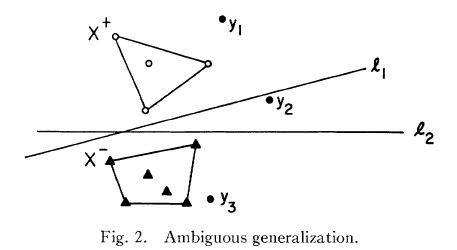
\includegraphics[height=4cm]{Cover1965-ambiguous}    
    \caption{Illustration of ambiguous assignments (from \cite{Cover1965})}
  \end{figure}

\begin{itemize}
\item Number of ambiguous assignments: $C_{(P,N-1)}$
\item for $P$ data points and linearly separable assignments on $P-1$ data points, there are still two choices left for the remaining data point.\\
{\it proof: supplementary material}
\end{itemize}
%%
\textbf{$\Rightarrow$ Fraction of ambiguous, linearly separable assignments}
\begin{equation}
	g_{(P,N)} \coloneqq \frac{ C_{(P,N-1)} }{
	 \underbrace{ C_{(P,N)}  }_{ \substack{\text{all linearly} \\ \text{separable assignments}}} }
\end{equation}
\begin{equation}
	g_{(\frac{P}{N})}^* = \underbrace{\lim_{P,N \rightarrow \infty}}_{
				\frac{P}{N} = \mathrm{const} }
	g_{(P,N)} = \left \{ \begin{array}{ll}
		1, 
			& \text{for } 0 \leq \frac{P}{N} \leq 2 \\\\
		\frac{1}{ \frac{P}{N} - 1},
			& \text{for } \frac{P}{N} > 2
	\end{array} \right.
\end{equation}
{\it proof: supplementary material}

\begin{figure}[h]
  \centering
\includegraphics[height=6cm]{section2_fig10}  
  \caption{fraction of ambiguous assignments}
\end{figure}


\paragraph{Interpretation:} \label{sec:interpretation} This means that
for $P/N>2$ learning is possible, i.e.\ a learned classifier
can make useful predictions.

% -----------------------------------------------------------------------------

\subsubsection{Conditions for Successful Learning with ERM}
Under which conditions one can learn with a specific model
($\rightarrow$ classifier) clearly depends on both the model and the
availability of data. The \emph{growth function} is an important tool
to describe this relation.

\emph{Capacity measures} quantitatively characterize a classifier and
we describe the \emph{VC-Dimension} which will further allow us to
derive bounds on the growth function.


\paragraph{General classification problems}\mbox{}\\
Observations: $\Big\{ \Big( \vec{x}^{(\alpha)}, y_T^{(\alpha)} \Big) \Big\}, \alpha = 1, \ldots, p$ \indent $\vec{x} \in \mathbb{R}^N, y_T \in \{-1,+1\}$\\\\
Set of classifiers: $y_{(\vec{x}; \vec{w})}$ \indent $y \in \{-1,+1\}$\\\\
Individual cost:
\begin{equation}
	Q_{(\vec{z};\vec{w})} = 1 - \delta_{y_T y} = 
	\left \{ \begin{array}{ll}
		0, & \text{if } y_{(\vec{x};{\vec{w})}} = y_T \\\\
		1, & \text{else}
	\end{array} \right. 
	\Rightarrow 0 - 1 \text{ loss}
\end{equation}
Model selection via ERM:
\begin{equation}
	R_{\emp [\vec{w}]}^{(p)} = \frac{1}{p} \sum_{\alpha = 1}^p 
		Q_{(\vec{z}^{(\alpha)};\vec{w})} \eqexcl \min
\end{equation}
\paragraph{Capacity measures for the set of classifiers}\mbox{}\\
Binary cost vector: $q_{(\vec{w})} = \Big( Q_{(\vec{z}^{(1)}, \vec{w})}, Q_{(\vec{z}^{(2)}, \vec{w})}, \ldots, Q_{(\vec{z}^{(p)}, \vec{w})} \Big)$\\
\indent $\Rightarrow$ different classifiers can induce the same cost vector on the training set 
\\\\
Number of different vectors $q_{(\vec{w})}$ induced by the whole set $\Lambda$ of classifiers:
\begin{equation}
	N_{ \underbrace{ (\vec{z}^{(1)}, \ldots, \vec{z}^{(p)}) }_{
		\substack{\text{training} \\ \text{set}}} }^{
			\overbrace{ \Lambda }^{
				\substack{\text{model} \\ \text{class}}}}
\end{equation}
\begin{itemize}
  \itR equivalent to the number of labelings (classification)
  induced by the set of classifiers on a given sample $\big(
  \vec{x}^{(1)}, \ldots, \vec{x}^{(p)} \big)$
  \itR $N_{(\vec{z}^{(1)}, \ldots, \vec{z}^{(p)})}^\Lambda \leq 2^p$
\end{itemize}
\textbf{Note:} General statements about the model class should not depend on the specific sample observed $\Rightarrow$ Need for a sample and distribution free quantity
\begin{equation} \tag{growth function}
	G_{(p)}^\Lambda = \ln \underbrace{ \bigg( 
		\sup_{\vec{z}^{(1)}, \ldots \vec{z}^{(p)}}
		N_{(\vec{z}^{(1)}, \ldots, \vec{z}^{(p)})}^\Lambda \bigg) }_{
			\text{worst case}}
\end{equation}
bound on the growth function
\begin{equation}
	G_{(p)}^\Lambda
	\left \{ \begin{array}{ll}
		= p \ln 2 
		& \text{for } p \leq \dvc \\\\
		\leq \dvc \Big( 1 + \ln \frac{p}{\dvc} \Big) 
		& \text{for } p > \dvc
	\end{array} \right.
\end{equation}
{\it proof: \textcite[ch.~4.10]{Vapnik1998}}
\begin{center}\includegraphics[height=8cm]{section2_fig11}
\end{center}
\textbf{Note:} While the number of potential labelings grows as $2^p$,
the growth function quantifies in how many different ways the data
could be labeled by the classifier. The higher the capacity of the
classifier, the more different labelings are possible.

\paragraph{$\dvc$: VC-dimension (\underline{V}apnik, \underline{C}hernovenkis)}
\begin{itemize}
	\item capacity measure for a given set of models 
	\item largest number of data points on which (at least for one set) 
		$2^p$ different loss vectors (i.e. label assignments) can be 
		induced
\end{itemize}
$\Rightarrow$ These results provide answers to the questions posed in chapter 2.1.1:
\begin{enumerate}[(1)]
\item {\bf Learnability} 
\begin{equation}
	P \bigg\{ \sup_{\vec{w} \in \Lambda} \Big| R_{(\vec{w})}
		- \underbrace{ R_{\emp (\vec{w})}^{(p)} }_{
			\frac{1}{p} G_{(p)}^\Lambda 
			\xrightarrow[p \rightarrow \infty]{} 0}
		\Big| > \eta	\bigg\} 
		\xrightarrow[p \rightarrow \infty]{\text{a.s.}} 0
\end{equation}
{\it proof: \textcite[ch.~14]{Vapnik1998}}
\\\\
Note: 
\begin{equation} \tag{original proof}
	\frac{1}{p} H_{(p)}^\Lambda \xrightarrow[p \rightarrow \infty]{} 0
\end{equation}
and
\begin{equation} \tag{'entropy'}
	H_{(p)}^\Lambda = \Big< \ln 
		N_{(\vec{z}^{(1)}, \ldots, \vec{z}^{(p)})}^{\Lambda} 
		\Big>_{\vec{z}}
\end{equation}
Inductive learning using the ERM method is only guaranteed (for large enough sample size) if $\dvc$ is finite. \slideref{example of an unlearnable problem}
\\\\
\item {\bf Finite samples: Bound on the generalization error}
\begin{equation}
	P \bigg\{ \sup_{\vec{w} \in \Lambda} \Big| R_{(\vec{w})}
		- R_{\emp (\vec{w})}^{(p)} \Big| > \eta \bigg\}
	< 4 \exp \bigg\{ G_{(2p)}^\Lambda - p 
		\Big( \eta -\frac{1}{p} \Big)^2 \bigg\}
\end{equation}
{\it proof: supplementary material}
\\\\
Note:
\begin{equation} \tag{original proof}
	G_{(2p)}^\Lambda \rightarrow \underbrace{ H_{\mathrm{ann}(2p)}^\Lambda }_{ \substack{
			\text{annealed} \\ \text{entropy} }}
		 = \ln 
		\Big< N_{(\vec{z}^{(1)}, \ldots, \vec{z}^{(p)})}^{\Lambda} 
		\Big>_{\vec{z}}
\end{equation}
and 
\begin{equation}
	H_{(2p)}^\Lambda \leq H_{\mathrm{ann} (p)}^\Lambda \leq G_{(p)}^\Lambda
\end{equation}
bound is non-trivial only if $G_{(2p)}^\Lambda$ sublinear in $p$
\begin{equation}
	\begin{array}{ll}
	G_{(2p)}^\Lambda - p \Big\{ \eta - \frac{1}{p} \Big\}^2
	& = p \Big\{ 2 \ln 2 - \Big( \eta -\frac{1}{p} \Big)^2 \Big\}
		> p \big\{ 2 \ln 2 - 1 \big\} \\\\
	& = 0.386p > 1
	\end{array}
\end{equation}
\item {\bf Finite samples: Deviation from the optimal model}
\begin{equation}
	P \Bigg\{ R_{(\vec{w}_p)} - R_{(\vec{w}_0)}
		> \Bigg\{ \frac{G_{(2p)}^\Lambda - \ln \frac{\epsilon}{8}}{p} 
		\Bigg\}^{\frac{1}{2}} 
		+ \bigg\{ -\frac{\ln \frac{\epsilon}{2}}{2p}
		\bigg\}^{\frac{1}{2}} + \frac{1}{p} \Bigg\} < \epsilon
\end{equation}
{\it proof: supplementary material}
\[ p \uparrow \left \{ \begin{array}{l}
	\epsilon \downarrow \text{ for equal bound on the difference} \\\\
	\text{bound on the difference } \downarrow \text{ for equal } \epsilon
\end{array} \right. \]
\end{enumerate}

\paragraph{Comments}
\begin{itemize}
  \itR bounds can be made tighter and condition on learnability made
  less strict if a capacity measure is used, which depends on the
  distribution $P_{(\vec{z})}$ (entropy or annealed entropy) \itR
  better bounds can be achieved using other capacity measures \itR
  regression problems can be treated in a similar manner if every
  continuous loss function $Q_{(\vec{z},\vec{w})}$ is replaced by a
  set of binary indicator functions
\end{itemize}
\begin{equation}
	I_{(\vec{z}, \vec{w}, \beta)} = \underbrace{ \theta_{\big( Q_{(\vec{z}, \vec{w})} 
		- \beta \big)} }_{ \substack{\text{step} \\ \text{function}}}, \beta \in \mathbb{R}
\end{equation}

% -----------------------------------------------------------------------------
\subsection{Support Vector Machines} \label{sec:SVM} While the bounds
derived from SLT are interesting from a theoretical
point of view, they more generally justify structural risk
minimisation as a guiding principle for model optimization.
 
Support Vector Machines (SVMs) provide an important example of a
learning approach that is based on structural risk minimization (SRM)
rather than ERM.

% -----------------------------------------------------------------------------
\subsubsection{Learning by Structural Risk Minimization}
Typical bound on the generalization error for ERM:
\begin{equation}
	P \bigg\{ \sup_{\vec{w} \in \Lambda} \Big| R_{(\vec{w})} 
		- R_{\emp (\vec{w})}^{(p)} \Big| > \eta \bigg\} 
	< \underbrace{ 4 \exp \bigg\{ G_{(2p)}^\Lambda - p 
		\bigg( \eta - \frac{1}{p} \bigg)^2 \bigg\} }_{
			\eqexcl \epsilon}
\end{equation}
In this formulation, $\eta$ depends on $\epsilon$. Therefore with
probability larger than $1 - \epsilon$ we obtain:
\begin{equation}
	R_{(\vec{w})} < R_{\emp (\vec{w})}^{(p)} + \Bigg\{
		\frac{G_{(2p)}^\Lambda - \ln \frac{\epsilon}{4}}{p}
		\Bigg\}^{\frac{1}{2}} + \frac{1}{p}
\end{equation}
{\it cf. supplementary material}
\begin{equation}
	R_{(\vec{w})} < \underbrace{ R_{\emp (\vec{w})}^{(p)} }_{ \substack{\text{empirical} 
		\\ \text{error}}} 
		+ \underbrace{C}_{
		\substack{ \text{complexity} \\ \text{term}}}
		, C = C_{(\dvc,P)}
\end{equation}

\begin{figure}[h]
  \centering
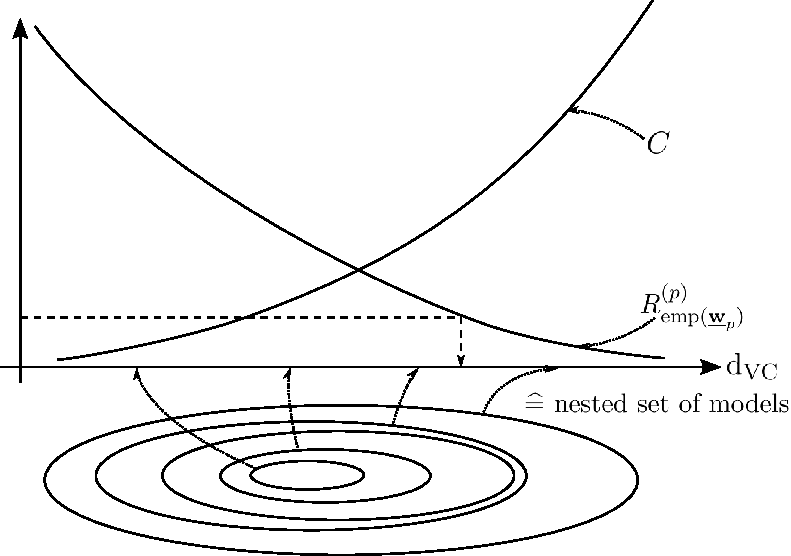
\includegraphics[height=6.5cm]{section2_fig12}  
  \caption{Illustration of the SRM approach: Inner to outer ellipses represent models of increasing capacity ($d_{VC}$). Models on the very left have low capacity and high training error ($\rightarrow$ underfitting), models on the right have high capacity and low training error ($\rightarrow$ overfitting).}
  \label{fig:SRM-principle}
\end{figure}


\paragraph{\underline{S}tructural \underline{R}isk \underline{M}inimization:}
\emph{Minimize capacity of the model class under the constraint, that the empirical error is not too large.}\\\\
$\Rightarrow$ Keeping empirical error fixed, $R_{(\vec{w})}$ can be optimized by minimizing the capacity $C$ of the model. 
\\\\
\textbf{Note:} SRM-learning is consistent ({\it see \cite[ch.~6.3]{Vapnik1998})}

% -----------------------------------------------------------------------------

\subsubsection{Application of SRM to Classification with Binary Connectionist Neurons}
Training data: $\Big\{ \Big( \vec{x}^{(\alpha)}, y_T^{(\alpha)} \Big) \Big\}, \alpha = 1, \ldots, p,$ \indent $\vec{x} \in \mathbb{R}^N, y_T \in \{-1,+1\}$\\\\
Connectionist neurons: $y = \sign \big( \vec{w}^T \vec{x} + b \big)$ 
\newpage					%NEWPAGE for visual reasons
\noindent Classification boundary:
\begin{equation} \tag{hyperplane}
	\vec{w}^T \vec{x} + b = 0
\end{equation}
\indent $\Rightarrow$ does not change if $\vec{w}^T$ and $b$ are multiplied by the same factor
\\\\
Canonical hyperplanes: 
\\\\
Data dependent normalization of $\vec{w}$ and $b$ such that:
\begin{equation}\label{eq:marginNormalization}
	\min_{\alpha = 1, \ldots, p} \Big| \underbrace{\vec{w}^T \vec{x}^{(\alpha)} + b}_{:=h}
		\Big| \eqexcl 1 
\end{equation}
For the closest data point, this sets the Normalized distance $d$ to
\[ \begin{array}{cl}
	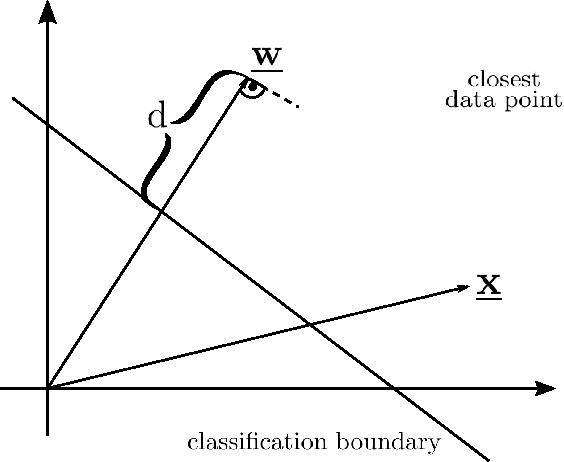
\includegraphics[height=6cm]{section2_fig13}
	& \mathrm{d} = \Big| 
		\underbrace{ \frac{ \vec{w}^T \vec{x} }{ |\vec{w}| }}_{
			\substack{ \text{length of} \\
				\text{projection of} \\
				\vec{x} \text{ on } \vec{w}}}
		+ \underbrace{ \frac{b}{|\vec{w}|} }_{
			\substack{ \text{distance from} \\
				\text{origin (} b \text{ is} \\
				\text{negative because} \\
				\text{origin in direction} \\
				- \vec{w}}}
		\Big| \\\\
	\mathrm{d} = \frac{1}{|\vec{w}|} 
		\underbrace{ \big| \vec{w}^T \vec{x} + b \big| }_{
			\eqexcl 1} = \frac{1}{|\vec{w}|} 
	& \text{''margin'' of a canonical hyperplane}
      \end{array} \] 
To apply the SRM principle, we need to construct a nested sequence of sets of models. These models are parametrised via their weights:
\begin{equation}
	|\vec{w}| \leq \mathrm{d}_{\mathrm{w}}^{-1}
\end{equation}
\begin{figure}[h]
  \centering
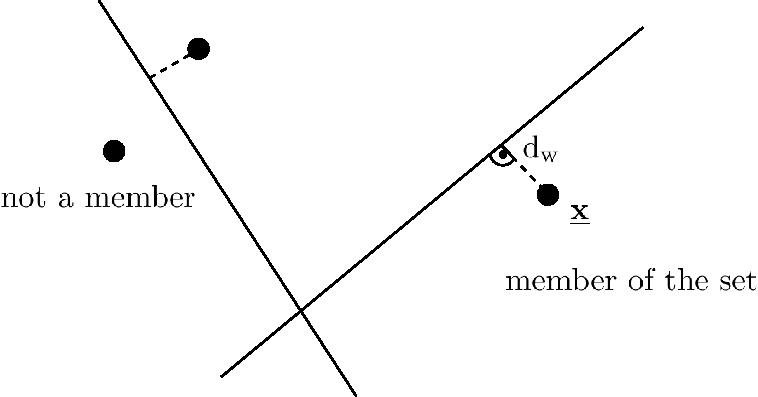
\includegraphics[height=4cm]{section2_fig14}
  \caption{Application of the SRM principle: Better figure???}
  \label{fig:applicationSRM}
\end{figure}

\begin{itemize}
  \itl for each value of $\vec{w}$, this yields a set of connectionist
  neurons with margin larger than $\mathrm{d}_{\mathrm{w}}$.  

  \itl sequence of numbers $\mathrm{d}_{\mathrm{w}}$ leads to a nested
  sequence of sets of models
\itl minimizing $|\vec{w}|$ corresponds to maximizing the margin
\end{itemize}
\textbf{Note:} Large $\mathrm{d}_{\mathrm{w}}$ means low capacity,
because some labelings cannot be induced. This relation between the
weight-dependent margin $d_\mathrm{w}$ and the capacity of the classifier is
quantified in the following theorem providing a bound on the
VC-Dimension.
\\\\
\textbf{Theorem:} Let $|\vec{x}| \leq R$ (bounded range of $\vec{x}$
for which $P_{(\vec{x})} \neq 0$), then:
\begin{equation}
	\dvc \leq \min \bigg( \bigg[ 
		\underbrace{ \frac{R^2}{\mathrm{d}_{\mathrm{w}}^2} }_{
				\text{New!}}
		\bigg], N \bigg) + \underbrace{1}_{
				\substack{ \dvc \text{of the} \\
					\text{connectionist} \\
					\text{neuron}}}
\end{equation}
{\it proof: \textcite[ch.~8.5]{Vapnik1998}}\\\\
\textbf{Note:} $\frac{R^2}{\mathrm{d}_{\mathrm{w}}^2}$ is independent
of the dimension $N$ of feature space
\begin{itemize}
  \itl VC-dimension of ''fat'' hyperplanes is independent of the
  number $N$ of parameters 

  \itl this provides an approach to learn classification in
  high-dimensional spaces that avoids overfitting
\end{itemize}


% -----------------------------------------------------------------------------

\subsubsection{SRM Learning for Linearly Separable Problems}
We now apply this approach to learn the weights of a connectionist
neuron (i.e.\ a linear classifier) assuming that data are linearly
separable.\\\\
\emph{Training data:}
\[ \Big\{ \Big( \vec{x}^{(\alpha)}, y_T^{(\alpha)} \Big) \Big\}, \alpha = 1, 
	\ldots, p, \text{\indent} \vec{x} \in \mathbb{R}^N, y_T \in \{-1, +1\}
\]
\subsubsection*{Model selection through SRM: Primal Problem}
\[ \begin{array}{ll}
	\frac{1}{2} |\vec{w}|^2 \eqexcl \min 
	& \text{minimization of model complexity} \\\\
	y_T^{(\alpha)} \Big( \vec{w}^T \vec{x}^{(\alpha)} + b \Big) \geq 1 \quad
		, \forall \alpha
\end{array} \]
\paragraph{Note:} The "$\geq 1$" guarantees correct classification of all training data points for the normalized margin of 1 (see eq.~\ref{eq:marginNormalization}).
\paragraph{Note:} This is a convex (quadratic!) optimization problem
$\leadsto$ only one (global!) minimum. There are standard (quadratic
programming) algorithms to find the solution!

\subsubsection*{Theorem by Kuhn and Tucker}
This theorem provides a strategy to efficiently solve the optimization
problem of finding the optimal weight vector $\vec{w}$. It links the 
solution for the original ("primal") problem to a "dual" problem which is often easier to solve (see below, generalization to nonlinear problems).
\paragraph{Preliminaries: } Consider
\begin{itemize}
\item $\vec{x} \in \mathrm{X} $ linear space $\mathrm{X}$ ($\leadsto$ Jensen's equality holds)
\item $A \subset \mathrm{X}$ where $A$ is a convex set 
\item $f_{k (\vec{x})}$ convex functions $f_k: \mathrm{X} \rightarrow \mathbb{R}, k = 0, \ldots, m$
\item $\exists \vec{x} \quad$ such that $f_{k (\vec{x})} < 0 \quad \forall k
  \in 1, \ldots, m$
\end{itemize}
The last point implies that there is a solution for which all constraints (formulated via the functions $f_{k (\vec{x})}$) can be fulfilled. \\
\paragraph{(primal) Optimization problem}\mbox{}\\
For $\vec{x} \in A$ find
\begin{equation}
	\underbrace{ f_{0 (\vec{x})} \eqexcl \min }_{\text{minimization}}
	\qquad \text{subject to} \qquad
			\underbrace{ f_{k (\vec{x})} \leq 0, k = 1, \ldots, m 
				}_{\text{constraints}}
\end{equation}
\paragraph{Lagrangian}
\begin{equation}
	L_{(\mathrm{x}, \{ \lambda_k \} )} \eqexcl f_{0 (x)}
	+ \sum_{k = 1}^m \underbrace{ \lambda_k }_{
		\substack{\text{lagrange} \\ \text{multipliers}}}
	\underbrace{ f_{k (\vec{x})} }_{\text{constraints}}
\end{equation}
\paragraph{Equivalent optimization problem} (existence of a saddle point):
\begin{equation}
	\min_{\mathrm{x} \in A} L_{(\mathrm{x}, \{ \lambda_k^*\})}
	= L_{(\mathrm{x}^*, \{ \lambda_k^* \})}
	= \max_{ \lambda_k \geq 0} L_{(\mathrm{x}^*, \{ \lambda_k \})}
\end{equation}
\begin{itemize}
\itR If the Lagrangian has such a saddle point, then $x^*$ is a solution to the constrained optimization problem and can be found by maximizing the right hand side with respect to the $\lambda_k$. 
\end{itemize}
\paragraph{Comments}
\begin{itemize}
	\itl violation of constraints 
	\begin{itemize}
		\itr $f_k$ positive 
		\itr maximization with respect to $\lambda_k$ leads to 
			divergence of $L$
		\itr minimization with respect to $\mathrm{x}$ assures, that
			constraints are fulfilled
	\end{itemize}
	\itl maximization with respect to $\lambda_k$
		\begin{center}
		$\lambda_k^f \neq 0$ only for values $\mathrm{x}^*$ for which
		the equality sign holds in the constraints
		\end{center}
\end{itemize}
\paragraph{Application of the theorem:}
\[ \begin{array}{ll}
	f_0: & \frac{1}{2} | \vec{w} |^2 \\\\
	f_\alpha: & - \Big\{ y_T^{(\alpha)} \Big( \vec{w}^T \vec{x}^{(\alpha)}
		+ b \Big) -1 \Big\} \leq 0
\end{array} \]
Lagrangian:
\begin{equation}\label{eq:lagrangianLinSep}
	L = \frac{1}{2} | \vec{w} |^2 
	- \sum_{\alpha = 1}^p \lambda_\alpha \Big\{ y_T^{(\alpha)} 
		\Big( \vec{w}^T \vec{x}^{(\alpha)} + b \Big) - 1 \Big\} 
\end{equation}
\[ \begin{array}{lll}
	\vec{w}, b: & \text{''primal variables''} 
		& \sim \text{ dimension of feature space} \\\\
	\lambda_\alpha: & \text{''dual variables''} 
		& \sim \text{ number of training data}
\end{array} \]\\\\
Finding the saddle point in 2 steps
\begin{enumerate}[(a)]
\item Minimization w.r.t. $\vec{w}$
\begin{equation}
	\begin{array}{ll}
	\frac{\partial L}{\partial \mathrm{w}_l}
	& 	= \mathrm{w}_l - \sum\limits_{\alpha = 1}^p \lambda_\alpha
		y_T^{(\alpha)} \mathrm{x}_l^{(\alpha)} \eqexcl 0 \\\\
	& \Rightarrow \underbrace{
		\vec{w} = \sum_{\alpha = 1}^p \lambda_\alpha 
		y_T^{(\alpha)} \vec{x}^{(\alpha)} }_{
			\substack{	\text{expansion of weight vector} \\
					\text{in terms of data points}}}
	\end{array}
\end{equation}
\item Minimization w.r.t. $b$:
\begin{equation}
	\frac{\partial L}{\partial b}
	= -\sum_{\alpha = 1}^p \lambda_\alpha y_T^{(\alpha)} \eqexcl 0
\end{equation}
\end{enumerate}
\emph{Problem:} the $\lambda_\alpha$ are unknown\\\\
$\Rightarrow$ inserting results into $L$ (eq.~\ref{eq:lagrangianLinSep}):
\begin{equation}
	\begin{array}{lcl}
	L & = & \frac{1}{2} \sum\limits_{\alpha,\beta = 1}^p \lambda_\alpha
		\lambda_\beta y_T^{(\alpha)} y_T^{(\beta)} 
		\Big( \vec{x}^{(\alpha)} \Big)^T \vec{x}^{(\beta)} \\\\
	&& -\sum\limits_{\alpha = 1}^p \lambda_\alpha y_T^{(\alpha)} 
		\sum\limits_{\beta = 1}^p \lambda_\beta y_T^{(\beta)} 
		\Big( \vec{x}^{(\beta)} \Big)^T \vec{x}^{(\alpha)} \\\\
	&& - \underbrace{ \Bigg( \sum\limits_{\alpha = 1}^p \lambda_\alpha 
			y_T^{(\alpha)} \Bigg) }_{ = 0 }
		b + \sum\limits_{\alpha = 1}^p \lambda_\alpha \\\\
	L & = & -\frac{1}{2} \sum\limits_{\alpha, \beta = 1}^p 
		\lambda_\alpha \lambda_\beta y_T^{(\alpha)}
		y_T^{(\beta)} 
		\underbrace{\Big( \vec{x}^{(\alpha)} \Big)^T 
			\vec{x}^{(\beta)}}_{ \circledast }
		+ \sum\limits_{\alpha = 1}^p \lambda_\alpha
	\end{array}
\end{equation}
this dual optimization problem is typically solved using SMO methods (see section \ref{sec:sequentialOptim}, software implementation: \texttt{libsvm}):
\begin{equation}
	L = \max \lambda_\alpha
\end{equation}
constraints:
\[ \begin{array}{l}
	\lambda_\alpha \geq 0, \alpha = 1, \ldots, p \\\\
	\sum\limits_{\alpha = 1}^p \lambda_\alpha y_T^{(\alpha)} = 0
\end{array} \]
If the Lagrange parameters $\lambda_\alpha$ are known, the weights are calculated as a linear combination of data points:
\begin{equation} \tag{calculation of $\vec{w}$}
	\vec{w} = \sum\limits_{\alpha = 1}^p \lambda_\alpha 
		y_T^{(\alpha)} \vec{x}^{(\alpha)}
\end{equation}
and $b$ can be calculated using the fact that
\begin{equation}
	y_T^{(\alpha)} \Big( \vec{w}^T \vec{x}^{(\alpha)} + b \Big) = 1
		\text{ for ''support vectors''}
\end{equation}
because $\lambda_\alpha \neq 0$ holds only for those data points (i.e.\ the support vectors)! {\it (cf. theorem by Kuhn and Tucker)}
\begin{equation}
	y_T^{(\alpha)} \sum\limits_{\beta = 1}^p \lambda_\beta 
		y_T^{(\beta)} \Big( \vec{x}^{(\beta)} \Big)^T
		\vec{x}^{(\alpha)} + y_T^{(\alpha)} b = 1
\end{equation}
\begin{equation}
	b = y_T^{(\alpha)} - \sum\limits_{\beta = 1}^p \lambda_\beta
		y_T^{(\beta)} \Big( \vec{x}^{(\beta)} \Big)^T 
		\vec{x}^{(\alpha)} 
\end{equation}
because $\big( y_T^{(\alpha)}\big)^2 = 1 $
\begin{equation} \tag{calculation of $b$}
	b = \frac{1}{\#_{\mathrm{SV}}} \sum\limits_{\mathrm{SV}}
		\bigg( y_T^{(\alpha)} - \sum\limits_{\mathrm{SV}}
			\lambda_\beta y_T^{(\beta)} 
			\underbrace{ \Big( \vec{x}^{(\beta)} \Big)^T 
			\vec{x}^{(\alpha)} }_{ \circledast }
		\bigg)
\end{equation}
Classification:
\begin{equation}
	\begin{array}{ll}
	y 
	& = \sign \big( \vec{w}^T \vec{x} + b \big) \\\\
	& = \sign \bigg\{ \sum\limits_{\mathrm{SV}} \lambda_\alpha 
		y_T^{(\alpha)} \underbrace{ \Big( \vec{x}^{(\alpha)}
			\Big)^T \vec{x} }_{ \circledast } + b \bigg\}
	\end{array}
\end{equation}
\textbf{Notes:} This classifier, together with aforementioned learning rules for $\lambda_\alpha$ and $b$, is called ''\emph{support vector machine}''.
\\\\
{\bf Comments}
\begin{itemize}
	\item only points on the margin are support vectors (i.e. fulfill 
		the equality sign of the constraint) 
		$\leadsto$ usually only few SVs
	\item classification boundary has equal distance between examples from
		class +1 and class -1
	\item learning and classification depends only on scalar products ($\rightarrow$ similarities) between
		data points ($\circledast$)
\end{itemize}

% -----------------------------------------------------------------------------

\subsubsection{SRM Learning for Non-linear Classification Boundaries}
\textbf{Idea:} Projection into a new feature space, where decision
boundaries are linear:
\begin{center} 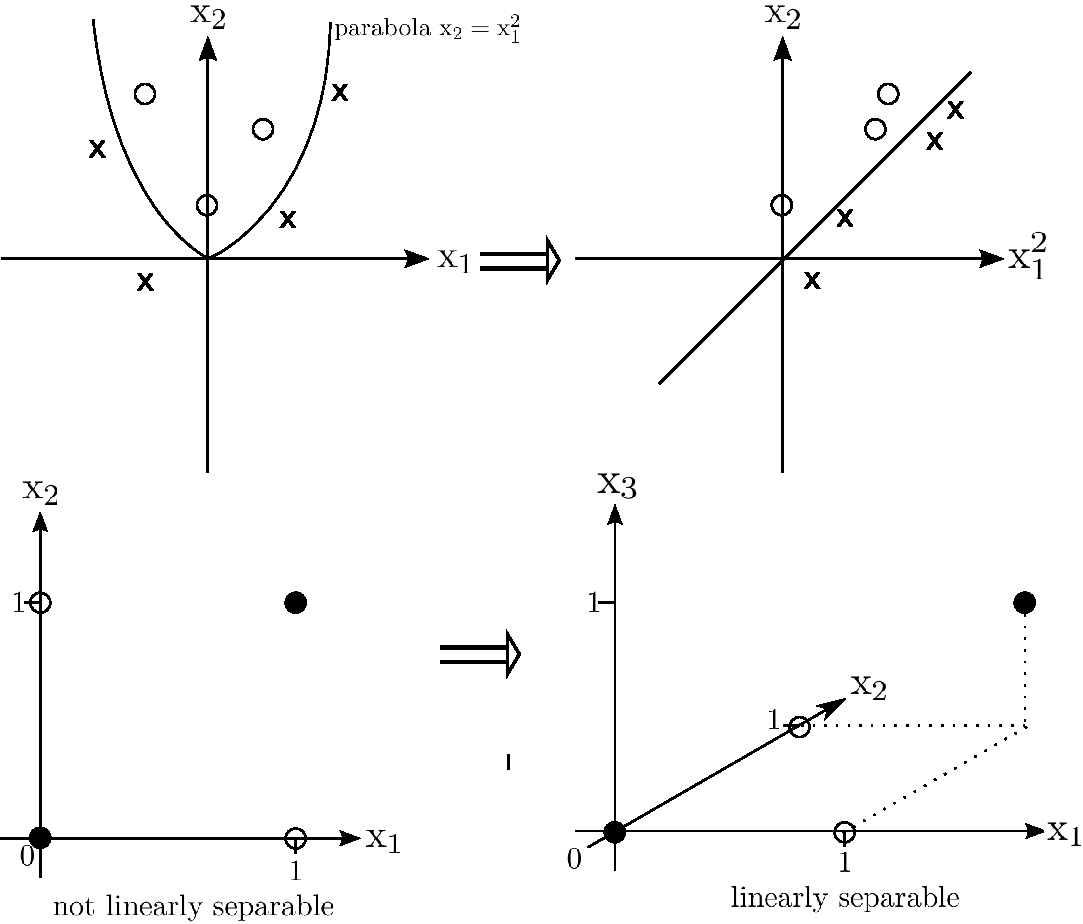
\includegraphics[height=10cm]{section2_fig15} \end{center}
{\bf Two steps}
\begin{equation} \tag{"intelligent" preprocessing}
	\underbrace{ \vec{x} }_{\substack{\text{elementary} \\
					\text{features} \\
					\text{(in } \mathbb{R}^N \text{)}}}
	\longrightarrow \underbrace{ \vec{\phi}_{(\vec{x})} }_{
			\substack{ \text{new feature space } F \\
				\text{(non-linear combination} \\
				\text{of elementary features}}}
\end{equation}
{\bf Kernel trick}
\begin{itemize}
	\itR avoid direct transformation $\vec{\phi}$
	\itR replace all scalar products by ''kernel functions''
	\[ \vec{\phi}_{(\vec{x})}^T \vec{\phi}_{(\vec{x}')} \rightarrow
		K_{(\vec{x}, \vec{x}')} \]
		Only scalar products are needed for SVM learning and 
		prediction.
              \itR under which conditions is this possible?
\end{itemize}

\paragraph{Mercer's theorem} establishes the important link between a
positive definite Kernel $K$ and a scalar product in some
corresponding metric feature space $F$. Given the following setting:
\[ \begin{array}{ll}
	\chi: & \text{compact subset of } \mathbb{R}^N \\\\
	K: \chi \times \chi \rightarrow \mathbb{R}, K \in L_\alpha,
		& \text{symmetric function (''kernel'')} \\\\
	\left. \begin{array}{l}
		T_k: L_{2 (\chi)} \rightarrow L_{2 (\chi)} \\\\
		\big( T_k f \big)_{(\vec{x})} \coloneqq \int\limits_\chi
			K_{(\vec{x},\vec{x}')} f_{(\vec{x}')}
			d \vec{x}
	\end{array} \right \} & \text{corresponding integral operator}\\\\
	\begin{array}{l}
		\lambda_j: \\\\
		\psi_j \in L_{2 (\chi)}:
	\end{array} & 
		\left. \begin{array}{ll}
			\text{eigenvalues} \\\\
			\text{normalized eigenfunctions}
		\end{array} \right \} \text{of } T_k
\end{array} \]
under the \emph{essential condition} for $T_k$ positive definite, i.e.\
\begin{equation}
	\int\limits_{\lambda \in \chi} K_{(\vec{x}, \vec{x}')} 
		f_{(\vec{x})} f_{(\vec{x}')} d \vec{x} d \vec{x}'
		> 0, \forall f \in L_{2 (\chi)}
\end{equation}
Mercers theorm then establishes that:
\begin{equation}
	\begin{array}{l}
	K_{(\vec{x}, \vec{x}')} = \sum\limits_{j = 1}^n \underbrace{\lambda_j
		\psi_{j (\vec{x})}  \psi_{j (\vec{x}')} }_{
			\substack{\text{eigenvalue} \\
				\text{decomposition}}} \\\\
	n \rightarrow \infty: \underbrace{ \text{absolute and uniform 
		convergence}}_{\text{non-trivial part}}
	\end{array}
\end{equation}
\textbf{Consequences of Mercer's theorem}
\begin{equation}
	\vec{\phi} : 
		\vec{x} \rightarrow \Big( \sqrt{\lambda_1} \psi_{1 (\vec{x})},
		\sqrt{\lambda_2} \psi_{2 (\vec{x})}, \ldots,
		\sqrt{\lambda_n} \psi_{n (\vec{x})},
		\Big)^T
\end{equation}
\begin{equation}
	K_{(\vec{x}, \vec{x}')} = \vec{\phi}_{(\vec{x})}^T 
		\vec{\phi}_{(\vec{x}')}
\end{equation}
{\bf Typical kernel functions}
\[ \begin{array}{ll}
	K_{(\vec{x}, \vec{x}')} = \big( \vec{x}^T \vec{x}' + 1 \big)^d
	& \text{polynomial kernel of degree } d \\
	& \rightarrow \text{ image processing: pixel correlations} \\\\
	K_{(\vec{x}, \vec{x}')} = \exp \Big\{ -\frac{(\vec{x} - \vec{x}')^2}{
		2 \sigma^2} \Big\}
	& \text{RBF-kernel with range } \sigma \\
	& \rightarrow \text{ infinite dimensional feature space} \\\\
	K_{(\vec{x}, \vec{x}')} = \tanh \big\{ \kappa \vec{x}^T \vec{x}' + \theta
		\big\}
	& \text{neural network kernel with parameters } \kappa \text{ and } \theta\\
	& \rightarrow \text{ not positive definite!} \\\\
	K_{(\vec{x}, \vec{x}')} = \frac{1}{ | \vec{x} - \vec{x}' + \epsilon
		|^N}
	& \text{Plummer kernel with parameter } \epsilon \\
	& \rightarrow \text{ scale invariant kernel}
\end{array} \]
Hyperparameter selection is typically done via cross-validation methods.

\paragraph{Comments}
\begin{enumerate}[(1)]
\item Kernel trick allows to work in high-dimensional feature space
  \[ K_{(\vec{x}, \vec{x}')} = \big( \vec{x}^T \vec{x}' + 1 \big)^{10}
  \leadsto \text{ space of all monomials up to a degree of } 10 \]
\item  SVMs vs. RBF-networks
\[ y_{(\vec{x})} = \sign \Big( \sum\limits_i \mathrm{w}_i 
	K_{(\vec{x}, \vec{x}')} \Big) \]
$\Rightarrow$ same architecture, but different learning rules\\
{\it (slide: Schoelkopf / Smola, figs. 7.7 \& 7.8)}

\item Mercer's theorem can be used to ''kernelize'' many different linear methods, both supervised or unsupervised. Important examples: 
\begin{itemize}
	\item Fisher discriminant analysis
	\item principal component analysis {\it (see MI 2)}
	\item K-means clustering \& self-organizing maps {\it (see MI 2)}
	\item canonical correlation analysis
\end{itemize}
\end{enumerate}
% -----------------------------------------------------------------------------

\subsubsection{The C-Support Vector Machine}
Many real-world problems are non-separable due to overlapping classes
or noise in the observation process. Given such a dataset, we might still find a feature-representation
allowing to obtain perfect prediction. Such a solution would, however,
not generalize well to new observations and therefore illustrates the
need to control overfitting in the SRM-framework.  The C-SVM
introduces a hyper-parameter $C$ to address this problem.

\begin{itemize}
	\itR empirical cost $R_{\emp}^{(p)} \neq 0$
	\itR trade-off between minimization of $R_{\emp}^{(p)}$ and capacity of 
		the model class
\end{itemize}
{\bf ''Primal'' problem}
\begin{equation}\label{eq:primal-problem-csvm}
	\begin{array}{ll}
	\frac{1}{2} |\vec{w}|^2 + \frac{C}{p} \sum\limits_{\alpha = 1}^p 
		\varphi_\alpha \eqexcl \min 
	& \begin{array}{l}
		\text{left: minimization of bound on VC dimension} \\
		\text{right: minimization of (approx.) margin error}
	\end{array}
	\end{array}
\end{equation}
Constraints:
\begin{equation}
	\begin{array}{ll}
		y_T^{(\alpha)} \Big( \vec{w}^T \vec{x}^{(\alpha)} + b \Big)
			\geq 1 - \varphi_\alpha
		& \substack{ \text{correct classification of all data points} \\
				\text{with margin } |\vec{w}| \text{ for } 
				\varphi = 0 } \\\\
		\varphi_\alpha \geq 0 
		& \text{''margin errors'' for } \varphi \neq 0
	\end{array}
\end{equation}
\begin{itemize}
	\itR exact margin error: $\frac{1}{p} \sum\limits_{\alpha = 1}^p 
		\theta_{(\varphi_\alpha)} \rightarrow$ NP hard optimization 
		problem
	\itR C: hyperparameter\footnote{Note: ``C'' here refers to a parameter in eq.~(\ref{eq:primal-problem-csvm}), not ``capacity'' directly, as in figure \ref{fig:SRM-principle}} $\leadsto$ model selection ($\leadsto$ crossvalidation).
	\itR Why margin error? $\leadsto$ margin necessary for bounding $\dvc$
		(i.e. to be smaller than $N$!)
\end{itemize}
{\bf Dual problem}
\begin{equation}
	-\frac{1}{2} \sum\limits_{\alpha,\beta = 1}^p \lambda_\alpha
		\lambda_\beta y_T^{(\alpha)} y_T^{(\beta)} 
		\underbrace{ \Big( \vec{x}^{(\alpha)} \Big)^T 
			\vec{x}^{(\beta)}}_{\text{kernel!}}
		+ \sum\limits_{\alpha = 1}^p \lambda_\alpha 
		\eqexcl \max_{(\lambda_\alpha)}
\end{equation}
Constraints:
\begin{equation}
	\begin{array}{l}
	0 \leq \underbrace{\lambda_\alpha \leq \frac{C}{p} }_{
		\substack{ \text{difference to linearly} \\
			\text{separable case}}} \\\\
	\sum\limits_{\alpha = 1}^p \lambda_\alpha y_T^{(\alpha)} = 0
	\end{array}
\end{equation}
{\it (derivation: see supplementary material)}
\begin{center} \includegraphics[height=5cm]{section2_fig16} \end{center}
Calculation of $\vec{w}$ and $b$:
\begin{equation}
	\vec{w} = \sum\limits_{\alpha = 1}^p \lambda_\alpha y_T^{(\alpha)}
		\vec{x}^{(\alpha)} 
	\leadsto \lambda_\alpha \neq 0 \text{ only for support vectors}
\end{equation}
let $SV_<$ be the $SV$s with $\lambda_\alpha < \frac{C}{p}$ ($SV$s on the margin)
\begin{equation}
	b = \frac{1}{\# SV_<} \sum\limits_{SV_<} \bigg( y_T^{(\alpha)}
		- \sum\limits_{SV} \lambda_\beta y_T^{(\beta)} 
		\underbrace{ \Big( \vec{x}^{(\beta)} \Big)^T 
			\vec{x}^{(\alpha)}}_{\text{kernel!}}
		\bigg)
\end{equation}
(via constraints of the primal problem)
\\\\
{\bf Classifier}
\begin{equation}
	y = \sign \big( \vec{w}^T \vec{x} + b \big) 
	= \sign \bigg( \sum\limits_{SVs} \lambda_\alpha y_T^{(\alpha)} 
		\underbrace{ \Big( \vec{x}^{(\alpha)} \Big)^T \vec{x}}_{
			\text{kernel!}}
		+ b
		\bigg)
\end{equation}

% -----------------------------------------------------------------------------

\subsubsection{Sequential Minimal Optimization}\label{sec:sequentialOptim}
Sequential Minimal Optimization (SMO) is an efficient procedure to
solve the dual problem.

The kernel matrix (or ''Gram matrix'') is defined as
\begin{equation} \tag{''Gram matrix''}
	K_{\alpha\beta} = K_{(\vec{x}^{(\alpha)}, \vec{x}^{(\beta)})}
\end{equation}
$$\begin{array}{c|ccccc}
  & 1      & 2      & 3      & \ldots & j      \\
  \hline
  1	& K_{11} & K_{12} & \ldots & \ldots & K_{1j} \\
  2 	& \vdots & \vdots & K_{23} & \ldots & K_{2j} \\
  \vdots 	& \vdots & \vdots & \vdots & \vdots & \vdots \\
  i	& K_{i1} & K_{i2} & \ldots & \ldots & K_{ij}
\end{array}
$$
and is typically pre-computed to speed up subsequent computations.

\begin{itemize}
	\itR SVMs operate on pairwise (similarity) data!
	\itR positive definite kernel
	\begin{itemize}
		\itr positive definite Gram matrix
		\itr well defined optimization problem
	\end{itemize}
\end{itemize}
Optimization of the Lagrangian $\rightarrow$ iterative procedure
\begin{itemize}
	\itr choose two Lagrange multipliers $\lambda_\gamma, \lambda_\delta$
	\itr optimize Lagrangian with respect to $\lambda_\gamma, 
		\lambda_\delta$ obeying constraints (keeping all other 
		$\lambda_\alpha$ fixed)
	\itR optimization with respect to two variables can be done analytically
\end{itemize}
{\bf Selection rules} $\rightarrow$ good heuristics are important
\\\\
\underline{K}arush-\underline{K}uhn-\underline{T}ucker conditions (KKT conditions)
\begin{equation}\label{eq:kkt-conditions}
	\Big[ \underbrace{ y_T^{(\alpha)} \Big( \vec{w}^T \vec{x}^{(\alpha)} 
				+ b \Big) -1 + \varphi_\alpha }_{
			\substack{ \text{constraint of the primal problem:} \\
				= 0 \text{ for all data points on and} \\
				\text{within the margin}}}
	\Big] 
		\underbrace{ \lambda_\alpha }_{
			\substack{ \text{Lagrange} \\
				\text{parameter} \\
				\text{of the} \\
				\text{dual problem}}}
	= 0
\end{equation}
% -------> BEGIN CODE
\begin{enumerate}
\item \verb|loop over all | $\lambda_\gamma$
      \verb| wich violate KKT-conditions|\\
      (and additional ''threshold''-conditions due to errors in
determination of $b$); typically done using the ``primal problem'' (\ref{eq:kkt-conditions}), i.e.\ pick $\lambda_\alpha$ for which \ref{eq:kkt-conditions}$\neq 0$
\item \verb|for picked | $\lambda_\gamma$ \verb|, select | $\lambda_\delta$
       \verb| in order to make ''large steps'|\\
       \verb| towards the optimum|\\
       (general heuristics)
% -------> END CODE
\end{enumerate}


Reduced optimization problem - Lagrangian C-SVM:
\begin{equation}
	\begin{array}{llll}
	& \frac{1}{2} \sum\limits_{\alpha \beta} \lambda_\alpha \lambda_\beta
		y_T^{(\alpha)} y_T^{(\beta)} K_{\alpha \beta} 
		- \sum\limits_\alpha \lambda_\alpha
	& \eqexcl & \min_{(\lambda_\alpha)} \\\\
	& \frac{1}{2} \bigg[ \lambda_\gamma^2 
		\underbrace{ \Big( y_T^{(\gamma)} \Big)^2 }_{= 1} 
		\alpha_{\gamma\gamma} + \lambda_\delta^2 
		\underbrace{ \Big( y_T^{(\delta)} \Big)^2 }_{= 1}
		\alpha_{\delta\delta} + 2 \lambda_\gamma \lambda_\delta
		y_T^{(\gamma)} y_T^{(\delta)} K_{\gamma\delta}
		\bigg]
	& & \\\\
		& + \lambda_\gamma \underbrace{ \bigg[
		\sum\limits_{\beta \neq \delta} \lambda_\beta 
		y_T^{(\gamma)} y_T^{(\beta)} K_{\gamma\beta} - 1
		\bigg] }_{C_\gamma}
	& & \\\\
		& + \lambda_\delta \underbrace{ \bigg[ 
		\sum\limits_{\beta \neq \gamma} \lambda_\beta 
		y_T^{(\delta)} y_T^{(\beta)} K_{\delta\beta} - 1
		\bigg] }_{C_\delta}
		+ \mathrm{const}_{(\lambda_\delta, \lambda_\gamma)}
	& \eqexcl & \min_{(\lambda_\delta, \lambda_\gamma)} \\\\
	\circledast & \frac{1}{2} \bigg[ \lambda_\gamma^2 
		Q_{\gamma\gamma} + \lambda_\delta^2 Q_{\delta\delta}
		+ 2 \lambda_\gamma \lambda_\delta
		\bigg] + C_\gamma \lambda_\gamma + C_\delta \lambda_\delta
	& \eqexcl & \min_{(\lambda_\delta, \lambda_\gamma)}
	\end{array}
\end{equation}
Constraints:
\begin{equation}
	\begin{array}{lll}
	\circledast & 0 \leq \lambda_{\gamma,\delta} \leq \frac{C}{p}
		& \text{''box constraints''} \\\\
	& \lambda_\gamma + \underbrace{ \frac{y_T^{(\delta)}}{
			y_T^{(\gamma)}}}_{s} \lambda_\delta 
		= \underbrace{ \frac{1}{y_T^{(\gamma)}} 
			\sum\limits_{\beta \neq \gamma, \delta} \lambda_\beta
			y_T^{(\beta)} }_{d}
		& \text{''equality constraint''} \\\\
	\circledast & \lambda_\gamma + s \lambda_\delta = d
	\end{array}
\end{equation}
{\it (slide: analytical solution of constrained optimization (Schoelkopf / Smola, p. 308))} \\
{\it (supplementary material: Pseudocode (Schoelkopf / Smola, p. 313))}
\\\\
Optimization software: libsvm-package
\begin{center}
\verb|http://www.csie.ntu.edu.tw/|$\sim$\verb|cjlin/libsvm|
\end{center}
$\Rightarrow$ also different variants, multiclass problems, support vector regression, one-class SVMs. 

\paragraph{Note on Validation: } SVMs implement the SRM principle and
therefore favor simple models with a small VC-Dimension. This helps to
avoid overfitting. Do we need to validate? Similar to other
classification algorithms, SVMs require to make decisions regarding
the exact architecture to use. For example, we need to choose shape
and parameters of the kernel and how to weight simplicity vs.\ penalty
for boundary intrusions via the parameter C. Typically, these choices
are based on available data and may therefore lead to
overfitting. Thus they need to be validated, e.g.\ using (nested)
crossvalidation with the 0-1 loss function.

% -----------------------------------------------------------------------------

\newpage					%NEWPAGE for visual reasons
\subsection{The P-SVM Ansatz}

% -----------------------------------------------------------------------------

\subsubsection{Shortcomings of Standard SVM-Approaches}
Scale sensitive solutions\\
{\it (slide: NC 18(6), p. 1472 ff., Fig. 2)}
\\\\
All data points related to margin errors are support vectors
\begin{itemize}
	\itR many support vectors for problems with overlapping classes
	\itR expansion of $\vec{w}$ is not as ''sparse'' as it could be (even
		for the same classification boundary)
\end{itemize}
\[ \begin{array}{ll}
	\includegraphics[height=5cm]{section2_fig17}
	& \begin{array}{l}
		\text{SVM-solution:} \\
		y_{(\vec{x})} = \sign \bigg( \sum\limits_{SVs} \lambda_\alpha
			y_T^{(\alpha)} \Big( \vec{x}^{(\alpha)} \Big)^T 
			\vec{x} + b \bigg) \\\\
		\text{but: for 2d and linear classifiers} \\
		\text{expansion into two data points would suffice}
	\end{array}
\end{array} \]
Only positive definite kernel functions / Gram matrices
\begin{itemize}
	\itR some ''interesting'' kernels cannot be used \\
		{\it (cf. sine-kernel for periodic distributions)}
		\[ K_{(\vec{x}^{(\alpha)}, \vec{x}^{(\beta)})} 
			= \sin \Big\{ \mathrm{w} \Big| 
			\vec{x}^{(\alpha)} - \vec{x}^{(\beta)} \Big| \Big\}
		\]
		here Gram matrix must have at least some negative eigenvalues
		(because: $T_\gamma \vec{K} = 0$)
	\itR structured objects: sometimes hard to assure positive definiteness
		of relational measure (kernels)
\end{itemize}

% -----------------------------------------------------------------------------

\subsubsection{The Primal Optimization Problem}
Training data: $\Big\{ \Big( \vec{x}^{(\alpha)}, y_T^{(\alpha)} \Big) \Big\},\alpha = 1, \ldots, p, \vec{x} \in \mathbb{R}^N, y_T \in \{-1, +1\}$ 
\\\\
Connectionist neurons: $ y = \sign \big( \vec{w}^T \vec{x} + b \big)$ 
\\\\
Capacity measure for the model class: $\dvc \leq \min \Big( \Big[ \frac{R^2}{d_{\mathrm{w}}^2} \Big], N \Big) + 1$ \\
{\it (cf. chapter 2.2.2) }
\newpage					%NEWPAGE for visual reasons
\noindent \textcircled{1} {\bf Scale invariant objective function}
\[ \begin{array}{ll}
	\includegraphics[height=4cm]{section2_fig18}
	& \begin{array}{l}
		\text{project all data into the subspace (Id) defined by }
		\vec{w} \\\\
		\Rightarrow \text{ smallest possible value for }
		\frac{R^2}{d_{\mathrm{w}}^2}
	\end{array}
\end{array} \] 
\begin{equation}
	R \rightarrow \widetilde{R} = \min\limits_{t \in \mathbb{R}} 
		\max\limits_\alpha \Big| \widehat{\vec{w}}^T
		\vec{x}^{(\alpha)} + t \Big|, 
	\widehat{\vec{w}} = \frac{\vec{w}}{|\vec{w}|} \text{ unit vector}
\end{equation}
\begin{equation}
	\begin{array}{lll}
	\frac{\widetilde{R}^2}{d_{\mathrm{w}}^2}  
	& = \vec{w}^2 \bigg\{ \min\limits_{t \in \mathbb{R}} \max\limits_\alpha
		\Big( \widehat{\vec{w}}^T \vec{x}^{(\alpha)} + t \Big)^2
		\bigg\}
	& \leq \vec{w}^2 \bigg\{ \max\limits_\alpha 
		\Big(\widehat{\vec{w}}^T \vec{x}^{(\alpha)} \Big)^2
		\bigg\} \\\\
	& = \max\limits_\alpha \Big( \vec{w}^T \vec{x}^{(\alpha)} \Big)^2
	& \leq \sum\limits_{\alpha = 1}^p \Big( \vec{w}^T
		\vec{x}^{(\alpha)} \Big)^2
	\end{array}
\end{equation}
New objective function:
\begin{equation}
	\sum\limits_{\alpha = 1}^p \Big( \vec{w}^T \vec{x}^{(\alpha)}
		\Big)^2 
	= \sum\limits_{\alpha = 1}^p \sum\limits_{i,j = 1}^N \mathrm{w}_i
		\mathrm{x}_i^{(\alpha)} \mathrm{w}_j 
		\mathrm{x}_j^{(\alpha)}
	= \sum\limits_{i,j = 1}^N \mathrm{w}_i
		\underbrace{ \bigg( \sum\limits_{\alpha = 1}^p 
			\mathrm{x}_i^{(\alpha)} \mathrm{x}_j^{(\alpha)}
			\bigg) }_{\substack{ p \cdot C_{ij} \\
				\text{correlation matrix} \\
				\text{of data} }}
			\mathrm{w}_j
\end{equation}
Matrix notation:
\begin{equation}
	\big| \vec{X}^T \vec{w} \big|^2 = \vec{w}^T \vec{X} \vec{X}^T \vec{w}
	= p \cdot \vec{w}^T \vec{C} \vec{w}, 
	\vec{X} = \Big( \vec{x}^{(1)}, \vec{x}^{(2)}, \ldots, \vec{x}^{(p)}
		\Big)
\end{equation}
Objective function is equivalent to the ''old'' SVM objective $|\vec{w}|^2$ if $\vec{C} = \vec{1}$ (i.e. for sphered data)
\\\\
\textcircled{2} {\bf New constraints}
$\leadsto$ applicability to general dyadic data

\includegraphics[height=4.5cm]{section2_fig19}

\begin{itemize}
\item selected complex features:
  $\Big\{ \vec{z}^{(\beta)} \Big\}, \beta = 1, \ldots, q$

\item measurement of feature values: $\Big( \vec{z}^{(\beta)} \Big)^T \vec{x}^{(\alpha)} \coloneqq K_{\beta \alpha} $\\
  $\leadsto q \times p$ matrix\footnote{Please note that this
    definition of $K$ corresponds to $K^T$ in
    \textcite{HochreiterObermayer2006}}
\end{itemize}
\paragraph{Quadratic cost function:}
\begin{equation}
	R_{\emp}^{(p)} = \frac{1}{2p} \sum\limits_{\alpha = 1}^p \Big( 
		\vec{w}^T \vec{x}^{(\alpha)} + b - y_T^{(\alpha)}
		\Big)^2
\end{equation}
\begin{itemize}
	\itR actually more natural for regression ratio than classification 
		problems
\end{itemize}
Constraints: minimal empirical error along the selected complex feature
\begin{equation} 
	\Big( \vec{z}^{(\beta)} \Big)^T \frac{\partial R_{\emp}^{(p)} }{
		\partial \vec{w}} = \frac{1}{p}
		\sum\limits_{\alpha = 1}^p 
		\underbrace{ \Big( \vec{z}^{(\beta)} \Big)^T 
			\vec{x}^{(\alpha)} }_{K_{\beta \alpha}}
		\Big( \vec{w}^T \vec{x}^{(\alpha)} + b - y_T^{(\alpha)}
		\Big) \eqexcl 0
\end{equation}
\begin{itemize}
	\itR one constraint per feature
\end{itemize}
\begin{equation}
	\frac{\partial}{\partial b} R_{\emp}^{(p)} 
	= \frac{1}{p} \sum\limits_{\alpha = 1}^p \Big( \vec{w}^T
		\vec{x}^{(\alpha)} + b - y_T^{(\alpha)}
		\Big) \eqexcl 0
\end{equation}
\begin{equation}
	\leadsto b = \frac{1}{p} \sum\limits_{\alpha = 1}^p 
		\Big( y_T^{(\alpha)} - \vec{w}^T \vec{x}^{(\alpha)} \Big)
\end{equation}
Normalization of $K_{\beta \alpha}$:
\begin{equation} 
	\begin{array}{lll}
		\frac{1}{p} \sum\limits_{\alpha = 1}^p K_{\beta \alpha} = 0
		& \text{zero mean} 
		& \text{because } \bigg( \frac{1}{p} \sum\limits_{\alpha = 1}^p
			K_{\beta \alpha} \bigg) b = 0 \\\\
		\frac{1}{p} \sum\limits_{\alpha = 1}^p K_{\beta \alpha}^2 = 1
		& \text{unit variance}
	\end{array}
\end{equation}
{\bf Primal problem of the P-SVM}
\begin{equation} 
	\frac{1}{2} \Big| \vec{X}^T \vec{w} \Big| \eqexcl \min
\end{equation}
Constraints: 
\begin{equation}
 	\vec{K} \Big\{ \vec{X}^T \vec{w} - \vec{y}_T \Big\} \eqexcl 0
\end{equation}
Offset $b$ is given by:
\begin{equation}
	b = \frac{1}{p} \sum\limits_{\alpha = 1}^p \Big( y_T^{(\alpha)} 
		- \vec{w}^T \vec{x}^{(\alpha)} \Big)
\end{equation}
but: if $\vec{K} = \big( K_{\beta \alpha} \big)$ has at least rank $p$ (no. of complex features equal or larger than number of data points), then constraints are always fulfilled with zero empirical error \\
\indent $\Rightarrow$ overfitting

% -----------------------------------------------------------------------------

\subsubsection{Regularization}
Trade-off between violation of constraints and minimization of capacity measure.
\\\\
Primal problem:
\begin{equation}
	\frac{1}{2} \Big| \vec{X}^T \vec{w} \Big|^2 + C \vec{1}^T 
	\big( \vec{\varphi}^+ + \vec{\varphi}^- \big) \eqexcl
	\min_{\big( \vec{w}, \vec{\varphi}^+, \vec{\varphi}^- \big)}
\end{equation}
Constraints:
\begin{equation} 
	\begin{array}{rll}
		\vec{K} \Big( \vec{X}^T \vec{w} - \vec{y}_T \Big) 
			+ \vec{\varphi}^+ + \epsilon \vec{1} 
		& \geq & 0 \\\\
		\vec{K} \Big( \vec{X}^T \vec{w} - \vec{y}_T \Big) 
			- \vec{\varphi}^- - \epsilon \vec{1} 
		& \leq & 0 \\\\
		\vec{\varphi}^+, \vec{\varphi}^- 
		& \geq & 0
	\end{array}
\end{equation}
{\bf C-regularization}
\begin{itemize}
	\itl violation of constraints for individual features (''outliers'')
	\itl large values for $\varphi_\beta^+$ and $\varphi_\beta^-
		\Rightarrow$ corresponding features influence the 
		classification boundary only weakly
\end{itemize}
{\bf $\epsilon$-regularization}
\begin{itemize}
	\itl deviations from the optimal residual error are tolerated if small
		enough (''small'' determined by value of $\epsilon$)
	\itl these features then do not influence the classification boundary
\end{itemize}

% -----------------------------------------------------------------------------

\subsubsection{Dual Formulation and P-SVM Classifier}
Lagrangian:
\begin{equation}
	\begin{array}{lllc}
	L 
	& = & \frac{1}{2} \vec{w}^T \vec{X} \vec{X}^T \vec{w} + 
		C \vec{1}^T \big( \vec{\varphi}^+ + \vec{\varphi}^- \big)
		& \text{cost function} \\\\
	&& \left. \begin{array}{l}
		- \big( \vec{\lambda}^+ \big)^T \Big\{
			\vec{K} \big( \vec{X}^T \vec{w} - \vec{y}_T \big)
			+ \vec{\varphi}^+ + \epsilon \vec{1} \Big\} \\\\
		+ \big( \vec{\lambda}^- \big)^T \Big\{
			\vec{K}\big( \vec{X}^T \vec{w} - \vec{y}_T \big)
			+ \vec{\varphi}^- - \epsilon \vec{1} \Big\}
	\end{array} \right \} & \substack{ \text{constraints for} \\
					\text{complex features} } \\\\
	&& - \big( \vec{\mu}^+ \big)^T \vec{\varphi}^+ - \big( \vec{\mu}^-
		\big)^T \vec{\varphi}^-
		& \substack{ \text{positivity of} \\
				\text{slack variables} }
	\end{array}
\end{equation}
Derivatives:
\begin{equation}
	\frac{\partial L}{\partial \vec{w}} = \vec{w}^T \vec{X} \vec{X}^T
		- \big( \vec{\lambda}^+ \big)^T \vec{K} \vec{X}^T
		+ \big( \vec{\lambda}^- \big)^T \vec{K} \vec{X}^T 
	\eqexcl 0
\end{equation}
\begin{equation}
	\vec{w}^T \vec{X} = \big( \vec{\lambda}^+ - \vec{\lambda}^- \big)
		\vec{K} = \big( \vec{\lambda}^+ - \vec{\lambda}^- \big)
		\vec{Z}^T \vec{X}
\end{equation}
Expansion of weight vector into ''support features'' rather than ''support data''. 
\begin{equation}
	\begin{array}{llll}
	\frac{\partial L}{\partial \vec{\varphi}^+} 
		= C \vec{1} - \vec{\lambda}^+ - \vec{\mu}^+ & \eqexcl \vec{0}
	& \leadsto & 
		\vec{\mu}^+ = C \vec{1} - \vec{\lambda}^+ \\\\
	\frac{\partial L}{\partial \vec{\varphi}^-}
		= -C \vec{1} + \vec{\lambda}^- + \vec{\mu}^- & \eqexcl \vec{0}
	& \leadsto & 
		\vec{\mu}^- = C \vec{1} - \vec{\lambda}^-
	\end{array}
\end{equation}
Derivation of the dual\footnote{Please note that here $K$ corresponds to $K^T$ in \textcite{HochreiterObermayer2006}} - inserting above equations into $L$: 
\begin{equation}
	\begin{array}{lll}
	L 
	& = & \frac{1}{2} \big( \vec{\lambda}^+ - \vec{\lambda}^- \big)^T
		\vec{Z}^T \vec{X} \vec{X}^T \vec{Z} \big( \vec{\lambda}^+ -
		\vec{\lambda}^- \big) + C \vec{1}^T \big( \vec{\varphi}^+
		+ \vec{\varphi}^- \big) 
		\\\\
	&& - \big( \vec{\lambda}^+ \big)^T \Big\{ \vec{K} \big( \vec{X}^T 
		\vec{Z} \big( \vec{\lambda}^+ - \vec{\lambda}^- \big) - 
		\vec{y}_T \big) + \vec{\varphi}^+ + \epsilon \vec{1} \Big\}
		\\\\
	&& + \big( \vec{\lambda}^- \big)^T \Big\{ \vec{K} \big( \vec{X}^T 
		\vec{Z} \big( \vec{\lambda}^+ - \vec{\lambda}^- \big) - 
		\vec{y}_T \big) - \vec{\varphi}^- - \epsilon \vec{1} \Big\}
		\\\\
	&& \big( C \vec{1} - \vec{\lambda}^+ \big)^T \vec{\varphi}^+ - 
		\big( C \vec{1} - \vec{\lambda}^- \big) \vec{\varphi}^-
		\\\\
	& = & - \frac{1}{2} \big( \vec{\lambda}^+ - \vec{\lambda}^- \big)^T \vec{K} 
		\vec{K}^T \big( \vec{\lambda}^+ - \vec{\lambda}^- \big)
		+ \big( \vec{\lambda}^+ - \vec{\lambda}^- \big) 
		\vec{K} \vec{y}_T 
		\\\\
	&& - \epsilon \big( \vec{\lambda}^+ - \vec{\lambda}^- \big)^T \vec{1}
		\eqexcl \max\limits_{(\vec{\lambda}^+, \vec{\lambda}^-)}
	\end{array}
\end{equation}
\begin{equation}
\frac{1}{2}	\big( \vec{\lambda}^+ - \vec{\lambda}^- \big)^T \vec{K} \vec{K}^T 
		\big( \vec{\lambda}^+ - \vec{\lambda}^- \big) - 
		\vec{y}_T^T \vec{K}^T \big( \vec{\lambda}^+ - \vec{\lambda}^-
		\big) + \epsilon \vec{1}^T \big( \vec{\lambda}^+ - 
		\vec{\lambda}^- \big) \eqexcl \min_{(\vec{\lambda}^+,
		\vec{\lambda^-})}
\end{equation}
\begin{itemize}
	\itR convex optimization problem for all $\vec{K}$
	\begin{itemize}
		\itl $\vec{K} \vec{K}^T$ is always positive (semi-)definite
	\end{itemize}
	\itR $\epsilon \vec{1}^T \big( \vec{\lambda}^+ - \vec{\lambda}^- 
		\big)$: sparseness constraint for the Lagrange multipliers
\end{itemize}
Evaluating the constraints we obtain (''box constraints''):
\begin{equation}
	\begin{array}{lll}
	\vec{0} \leq \vec{\lambda}^+ \leq C \vec{1},
	& \text{because } \vec{\mu}^+ \geq \vec{0} 
	& \leadsto C \vec{1} - \vec{\lambda}^+ \geq \vec{0} 
	\\\\
	\vec{0} \leq \vec{\lambda}^- \leq C \vec{1},
	& \text{because } \vec{\mu}^- \geq \vec{0} 
	& \leadsto C \vec{1} - \vec{\lambda}^- \geq \vec{0}
	\end{array}
\end{equation}
Optimization: adapted SMO method
\begin{center}
\verb|http://ni.cs.tu-berlin.de/software/psvm/index.html|
\end{center}
{\bf P-SVM classifier}
\begin{equation} 
	\begin{array}{ll}
	y & = \sign \big( \vec{w}^T \vec{x} + b \big) \\\\
	& = \sign \Big\{ \big( \vec{\lambda}^+ - \vec{\lambda}^- \big)^T
		\vec{Z}^T \vec{x} + b \Big\} \\\\
	\end{array} 
\end{equation}
\begin{equation}
	y_{\mathrm{x}} = \sign \Bigg\{ \sum\limits_{\beta \in \mathrm{SV}^+}
		K_{\beta \mathrm{x}} \lambda_\beta^+ - 
		\sum\limits_{\beta \in \mathrm{SV}^-} 
		K_{\beta \mathrm{x}} \lambda_\beta^-
		+ b \Bigg\}
\end{equation}
where: 
\begin{equation}
	\begin{array}{ll}
	b 
	& = \frac{1}{p} \sum\limits_{\alpha = 1}^p \Big( y_T^{(\alpha)}
		- \vec{w}^T \vec{x}^{(\alpha)} \Big) \\\\
	& = \frac{1}{p} \sum\limits_{\alpha = 1}^p \bigg( y_T^{(\alpha)}
		- \sum\limits_{\beta = 1}^q \big( \lambda_\beta^+
			- \lambda_\beta^- \big) \big(\vec{Z}^{(\beta)}
			\big)^T \vec{x}^{(\alpha)} \bigg) \\\\
	& = \underbrace{ \frac{1}{p} \sum\limits_{\alpha = 1}^p }_{
				\eqexcl 0 }
		\bigg( y_T^{(\alpha)} - \sum\limits_{\beta = 1}^q 
			\big( \lambda_\beta^+ - \lambda_\beta^- \big)
			\underbrace{ K_{\beta \alpha} }_{
				\eqexcl 0 }
			\bigg) \\\\
	& = \frac{1}{p} \sum\limits_{\alpha = 1}^p y_T^{(\alpha)}
	\end{array}
\end{equation}


% -----------------------------------------------------------------------------

\subsubsection{The Kernel Trick}
Under fairly mild assumptions {\it (cf. Hochreiter \& Obermayer(2006), New. Comp. 18, 1427ff, Appendix)} one obtains:
\begin{equation}
	\begin{array}{llll}
	\vec{\psi}: & \underbrace{\mathrm{z}}_{\substack{\text{from a} \\ \text{Hilbert space}}} 
		& \rightarrow & \underbrace{\vec{\psi}_{(\mathrm{z})}}_{ \text{from } l^2} \\\\
	\vec{\phi}: & \underbrace{\mathrm{x}}_{\substack{\text{from a} \\ \text{Hilbert space}}} 
		& \rightarrow & \underbrace{\vec{\phi}_{(\mathrm{x})}}_{ \text{from } l^2} \\\\
	K: & \mathrm{z}, \mathrm{x} & \rightarrow & K_{(\mathrm{z},
							\mathrm{x})}
	\end{array}
\end{equation}
then:
\begin{equation}
	\underbrace{ K_{(\mathrm{x}, \mathrm{z})} }_{\text{kernel}}
	= \underbrace{ \vec{\psi}_{(\mathrm{z})}^T \vec{\phi}_{(\mathrm{x})} }_{
		\text{scalar product}}
\end{equation}

% -----------------------------------------------------------------------------

\subsubsection{Properties of the P-SVM}
General dyadic data:
\[ \begin{array}{l|l}
				& \text{objects (attributes to be predicted)} \\
	\hline	
	\text{descriptions} 	& \text{Gram matrix}
\end{array} \]
\[\begin{array}{lcccc}
	\text{examples:} & \text{objects} && \text{descriptions} \\
	& \Downarrow && \Downarrow \\
	\text{DNA microarrays} & \text{probes} & \text{vs.} & \text{genes} \\
	\text{documents} & \text{text} & \text{vs.} & \text{indexwords}\\
	\text{web-pages} & \text{page} & \text{vs.} & \text{links}
\end{array} \]
\begin{itemize}
	\itR arbitrary rectangular Gram matrices
	\itR non-definite (square) matrices
	\itR Gram matrix measured or constructed
\end{itemize}
{\it slide: NC paper, Tab.3}
\\\\
Standard metric data: indefinite kernels:\\
e.g.: sine-kernel 
\[ K_{(\vec{x}, \vec{x}')} = \sin \big\{ 
	\theta \big| \vec{x} - \vec{x}' \big| \big\}
\]
{\it slide: NC paper, Fig. 4}
\\\\
Feature selection:
\begin{itemize}
	\itR ''support features'' are important for prediction
	\itR sparse set of support features (determined via regularization 
		parameter $\epsilon$)
	\itR binary classification problem
		\[ \begin{array}{ll}
			\lambda_\beta^+ \neq 0: 
			& \text{features supporting class ''}+1\text{''} \\
			\lambda_\beta^- \neq 0: 
			& \text{features supporting class ''}-1\text{''} 
		\end{array} \]
	\itR Lagrange parameters are directly related to the increase in 
		empirical error when one feature is removed
		({\it proof: see supplementary material})
		\[ \Delta_\gamma \coloneqq
			R_{\emp[\vec{w} - \lambda_\gamma \vec{z}^{(\gamma)}
			,b]}^{(p)}  - R_{\emp [\vec{w},b]}^{(p)} \leq 
			\frac{\epsilon | \lambda_\gamma | }{p}
			+ \frac{\lambda_\gamma^2}{2}
		\]
	\itR P-SVM is an example of a wrapper method for feature selection\\
		{\it slide: NC paper, Tab. 7}
\end{itemize}

% -----------------------------------------------------------------------------
